\ifx\wholebook\relax\else
\input{../Common.tex}
\input{../macroes.tex}
\begin{document}
\fi


\chapter{Fun with Robots}\label{cha:custo}

\begin{chapterfigure}
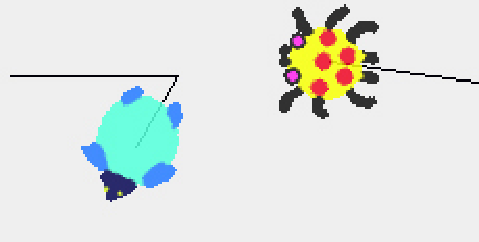
\includegraphics{beasts}
\end{chapterfigure}

The basic look of the robots is rather simple. In this chapter I show you how you can change the shape, the pen size and the color of robots. I present how you can draw yourselves the way your robots look like. For example your robot can look like an animal or a monster.  



\section{Robot Handles}
In addition to the fact that we can send messages to robot by clicking on them, you can have access to 
other functionalities such as duplicating, moving, or changing the look of your robot. These extra functionalities are available via handles that you get when you left-click on a robot. The handles are the round little icons around the robot as shown in Figure~\ref{fig:allHandles}. I will explain the functionalities when needed. Note that if you let your mouse over a handle a balloon will pop up and explain you its purpose. For now try to duplicate the robot by clicking on the green handle, move it by clicking on the black or destroy it using the pink pale crossed handle. 

\begin{figure}[h]
\begin{center}
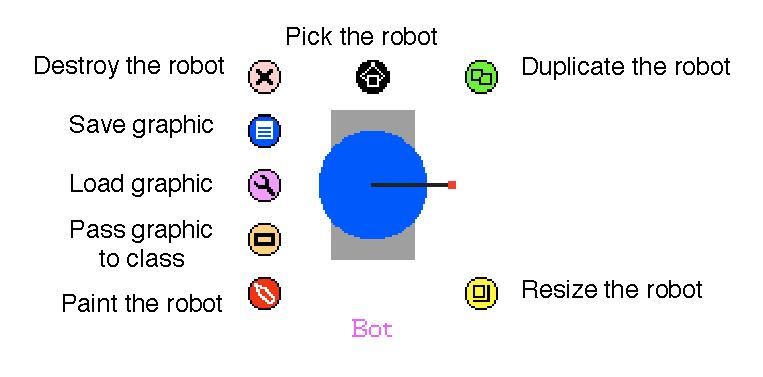
\includegraphics[width=8cm]{picaAllHaloAnnotated} 
\end{center}
\caption{Right-click to get the handles. \label{fig:allHandles}}
\end{figure}

\section{Pen Size and Color}
So far the trace left by our robot was black. However, you can change the color of a robot's pen by sending a robot the message \ct{penColor:} \index{penColor: aColor} with a color. For example the expression \ct{\caro penColor: Color blue} changes the color of the pen to blue. One of the ways to create a color is to send a message with the name of a color to the class \ct{Color}, such as \ct{Color blue} or \ct{Color yellow}. We will explain colors in the following section.

We can also change the thickness of the robot's pen by sending the message \index{penSize:}\ct{penSize:} with a number as argument, for instance \ct{\caro penSize: 5} make the pen to be 5 pixels wide.

Script~\ref{scr:blueLine} draws a thick blue line of 5 pixel width. Script~\ref{scr:Stair} draws a strange staircase by repeatedly increasing the pen size.

\begin{scriptwithtitle}{A blue line}\label{scr:blueLine}
| \caro |
\caro := \Turtle new.
\caro \textbf{penColor: Color blue}.
\caro go: 100.
\caro \textbf{penSize: 5}.
\caro go: 100
\end{scriptwithtitle}


\ 


\begin{scriptfig}{turtleMPenSize}{Stair}\label{scr:Stair}
| \caro |
\caro := \Turtle new.
\caro go: 40.
\textbf{\caro penSize: 2.}
\caro go: 40.
\textbf{\caro penSize: 4.}
\caro go: 40.
\textbf{\caro penSize: 6.}
\caro go: 40.
\end{scriptfig}

\ 

Changing the color of the robot itself is also possible using the
method \index{color: aColor}\ct{color:}. For instance, the expression \ct{\caro color: Color yellow} changes the color of  the robot to yellow. \scriptref{scr:yellowturtle} asks \ct{daly} to change its color and go forward, while \caro does not move and keep its default color.

\begin{scriptwithtitle}{Two Robots}\label{scr:yellowturtle}
| \caro daly |
\caro := \Turtle new.
daly  := \Turtle new.
daly color: Color yellow.
daly go: 100.
\end{scriptwithtitle}




\section{About Colors}

As previously mentioned already, \sq  is an environment built from and using objects. Therefore programming in \sq amounts to creating objects and sending them messages. In particular a \emph{color} is an object created by the class \ct{Color}. To get a color you  send a message to the class \ct{Color}. 


Some color messages are named for the color they get. For example, \ct{Color red} creates the color red. Here is the list of the predefined color name messages that you can send  to the class \ct{Color} to create that color: 
\ct{black}, \ct{veryVeryDarkGray}, \ct{veryDarkGray}, \ct{darkGray}, \ct{gray}, \ct{lightGray}, \ct{veryLightGray}, \ct{veryVeryLightGray}, \ct{white}, \ct{red}, \ct{yellow}, \ct{green}, \ct{cyan}, \ct{blue}, \ct{magenta}, \ct{brown}, \ct{orange}, \ct{lightRed}, \ct{lightYellow}, \ct{lightGreen}, \ct{lightCyan}, \ct{lightBlue}, \ct{lightMagenta}, \ct{lightBrown}, \ct{lightOrange}, \ct{paleBuff}, \ct{paleBlue}, \ct{paleYellow}, \ct{paleGreen}, \ct{paleRed}, \ct{veryPaleRed}, \ct{paleTan}, \ct{paleMagenta}, \ct{paleOrange}, and \ct{palePeach}.

You can also make a color by telling the \ct{Color} factory how to make it by mixing red, green and blue.  \scrref{scr:colorCreation} shows how to create colors this way using the method \index{r:g:b:}\ct{r: red g: green b: blue}. 
 The arguments of method \ct{r:g:b:} should be decimal numbers between 0 and 1.0. For example the expression \ct{Color r: 1 g: 0 b: 0} creates the same pure red color that you get from \ct{Color red}. 
 
 Finally the method \index{fromUser}\ct{fromUser} 
 lets you pick a color from a palette on the screen, and then shows you that color's ingredients. For that you need to execute the expression \ct{Color fromUser} using the \menu{print it} menu to get the result of the selection printed. Print the result by using the \menu{print it} menu when executing the expression \ct{Color fromUser}.

\begin{scriptfig}{colorFromUser}{Other ways to create colors}\label{scr:colorCreation}
"Produce a pure red"
Color r: 1 g: 0 b: 0

"Produce a light gray"
Color r: 0.1 g: 0.1 b: 0.1

"To choose your color from a palette"
Color fromUser
\end{scriptfig}


\section{Changing Robot Shape}
Another aspect of a robot that you can change is its shape. Two different shapes -- a circle, and a triangle  are built into the \ct{Bot} factory. But you can also draw the robot shape with a drawing tool as shown later in Section~\ref{sec:drawingTurtle}.

\begin{figure}[h]
\begin{center}
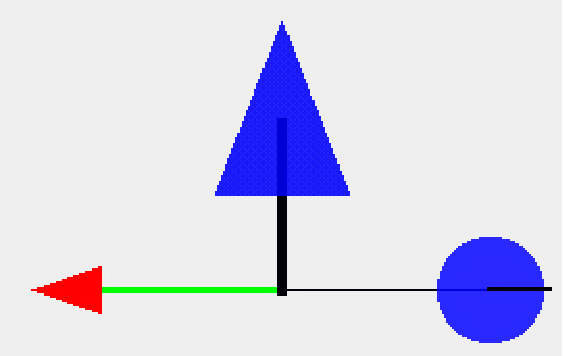
\includegraphics[width=8cm]{shapeAndSize}
\caption{Different robot shapes and sizes. \label{fig:shapeAndSize}}
\end{center}
\end{figure}

\scrref{scr:differentsize} shows how to change the shape of a robot as shown in Figure~\ref{fig:shapeAndSize}. The message \index{lookLikeTriangle} \ct{lookLikeTriangle} gives a triangular shape to a robot. The message \index{lookLikeCircle} gives a circular shape to a robot. The default shape is produced by sending the message  \index{lookLikeBot} \ct{lookLikeBot}. 

\begin{scriptwithtitle}{Creating Robots of Different Sizes and Shapes}\label{scr:differentsize}
| \caro daly  big\caro |
\caro := \Turtle new.
\caro \textbf{lookLikeTriangle}.
\caro west.
\caro color: Color red.
\caro penColor: Color green.
\caro penSize: 3.
\caro go: 100.
daly := \Turtle new.
daly \textbf{extent: 60@60}.
daly east.
daly go: 100.
big\caro := \Turtle new.
big\caro \textbf{lookLikeTriangle}.
big\caro \textbf{extent: 100@150}.
big\caro penSize: 5.
big\caro north.
big\caro go: 80.
\end{scriptwithtitle}


\paragraph{Robot Size.} The second aspect you can change is the size of a robot using the message \index{extent:} \ct{extent: widthAndHeight}, where the values of widthAndHeight represent the width and height of the rectangle in which the robot is drawn.  The argument \ct{widthAndHeight} is a pair of numbers also called a point in \sq. It is composed of two numbers separated by the \ct{@} symbol. For example, the point \ct{50@100} represents a rectangle of 50 pixels by 100.







\begin{figure}[h]
\begin{center}
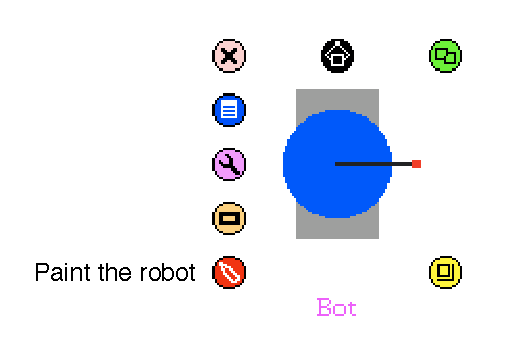
\includegraphics[width=6cm]{picaHaloAnnotated} 
\end{center}
\caption{Right-click to get the handles. \label{fig:paintToolCaroFlap} Getting the painting editor from the red handle.}
\end{figure}


\section{Drawing Your Own Robot}\label{sec:drawingTurtle}
\sq lets you  draw the robot itself and get robots that look like the  figure in the heading of this chapter. Now we describe step by step how you can draw your own robot. 

\paragraph{Step1. Getting the Painting Tool via the red Handle.}
The first step is to open the painting tool that is included in \sq. 
Right click or press command and click for Mac to get the halos around the robot you want to paint as shown by Figure~\ref{fig:paintToolCaroFlap}. Click on the red handle with the pen inside. This should open the paint tool shown in Figure~\ref{fig:paintOpen}. Do not worry about the other handle right now I explained them just after. 
Note that if you already drew a graphic, the graphic will be shown inside the painting tool. 


%\begin{figure}
%\begin{center}
%\includegraphics[width=6cm]{widgetFlaps} \includegraphics[width=6cm]{paint}  
%\end{center}
%\caption{Left: The widget flap. \label{fig:Paint} Right: Getting the painting \replace{editor}{tool} from the widget flap. \label{fig:widgetFlap}}
%\end{figure}

%\begin{figure}
%\begin{center}
%\includegraphics[width=5cm]{gettingPaintEditor}
%\end{center}
%\caption{Getting the painting \replace{editor}{tool} from the object palette. \label{fig:gettingPaintEditor}}
%\end{figure}

\begin{figure}[h]
\begin{center}
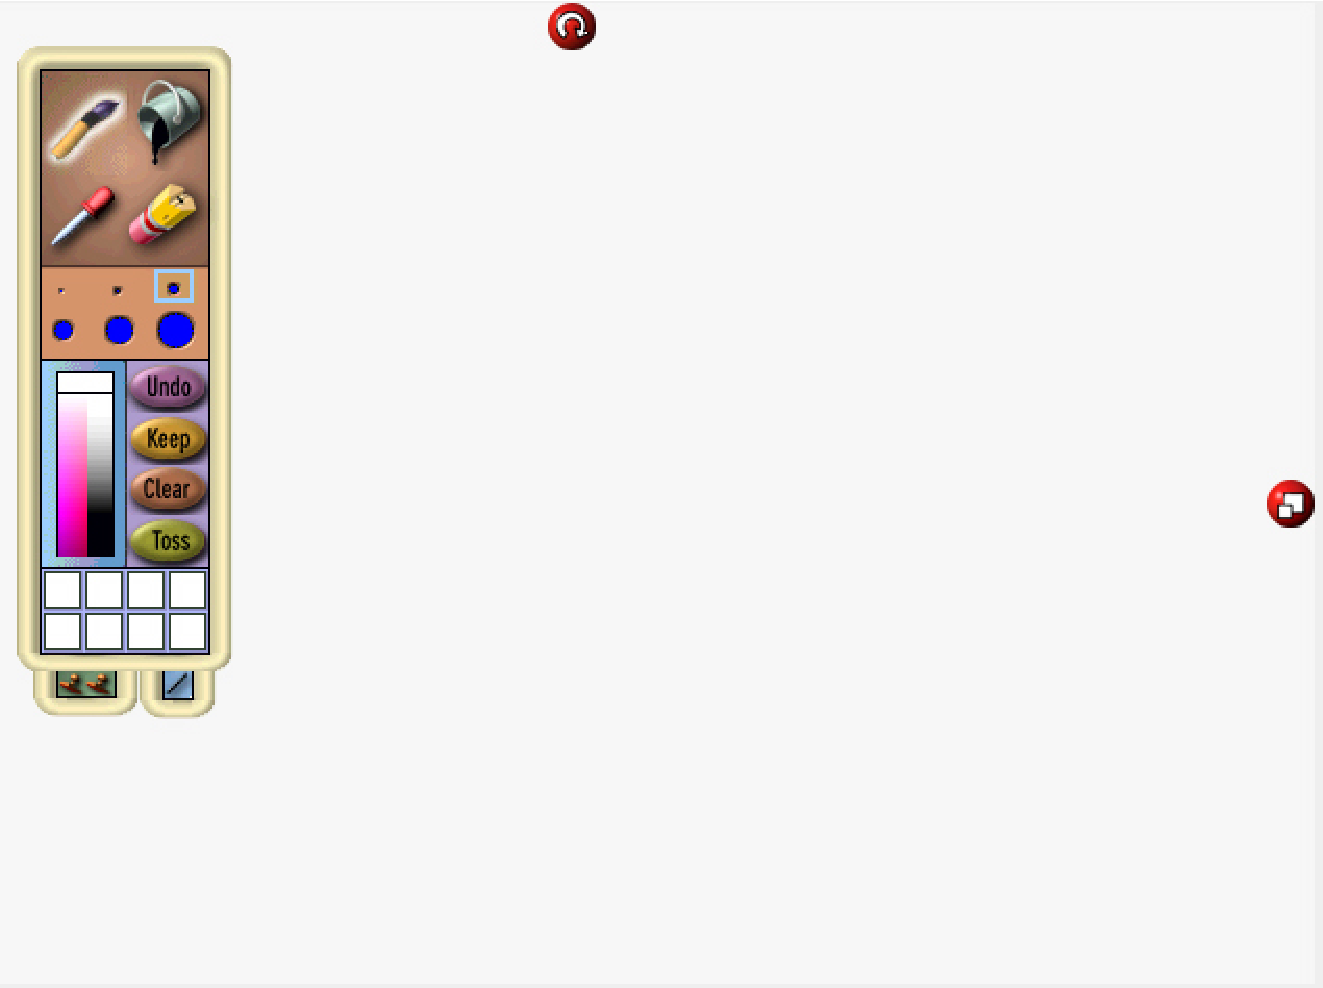
\includegraphics[width=14cm]{paintOpen}
\caption{The opened painting editor. \label{fig:paintOpen}}
\end{center}
\end{figure}

\newpage

\paragraph{Step2. Drawing the New Graphic.} The second step is to draw a new graphic for your robot. Draw your robot pointing to the right, as shown in Figure~\ref{fig:palette}. The painting editor has the usual features like choosing the brush size, filling a region, repeating a selected region, and selecting the painting color. The painting tool also has two buttons (shown in Figure~\ref{fig:rotate})  to rotate and zoom your drawing. 

\begin{figure}[h]
\begin{center}
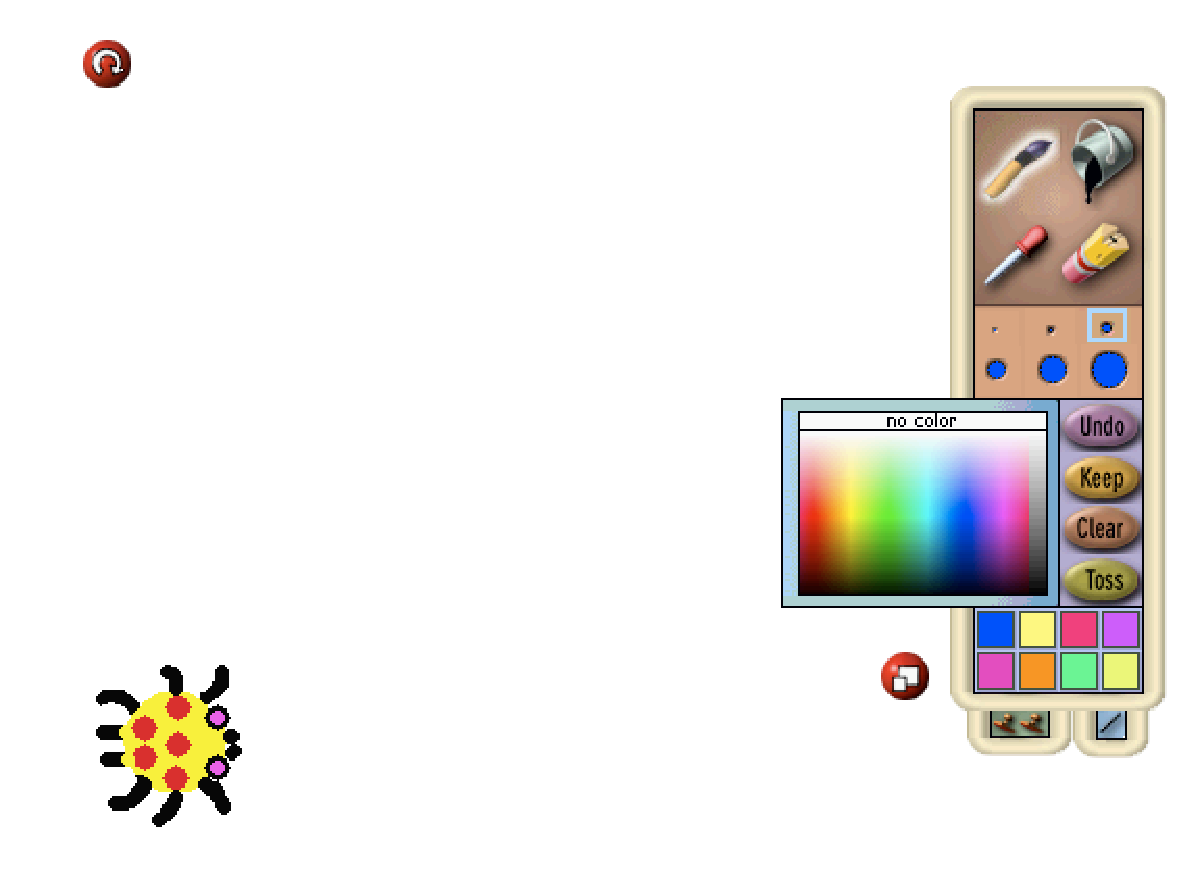
\includegraphics[width=12cm]{editingSpider}
\end{center}
\caption{Drawing a cool spider. \label{fig:palette}}
\end{figure}

\begin{figure}[h]
\begin{center}
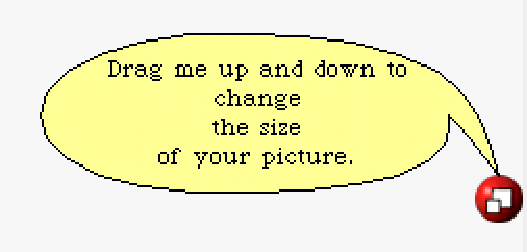
\includegraphics[width=5cm]{zoomButton} 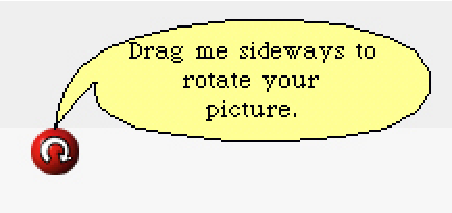
\includegraphics[width=5cm]{rotateButton}
\end{center}
\caption{The zoom and rotate buttons. \label{fig:zoom}\label{fig:rotate}}
\end{figure}


%\begin{figure}[h]
%\begin{center}
%
\includegraphics{spider} 
%\end{center}
%\caption{The robot is now looking like a spider and is pointing to the right. \label{fig:luth}}
%\end{figure}

\paragraph{Step3. Keeping the Graphic.} Once you are satisfied with your drawing, you should press the button \button{keep}. This closes the painting tool and your robot know is looking like graphic. Note that you can still get the other shapes such as the robot, the triangle or the circle sending the messages I presented above. 


\section{Saving and Restoring Graphics}\label{sec:saveturtle}
Once you have spent lot of time in drawing a robot, you can save it on a file. This way you will be able to load it in several environments, to exchange it with friends and you can to build a library of graphics over time. I will show you now how load save and load a graphic, then I will show how you can associate a graphic to a single robot or to a class so that all the newly created robots will look like the graphics you drew. I will start by showing you how to do all these manipulations by interacting with the robots directly but also how we can write scripts to do that automatically. 


\subsection{Using Handles}

\begin{figure}[h]
\begin{center}
\includegraphics{PicaHaloSaveAndLoadAnnotated}
\end{center}
\caption{The robot is now looking like a spider and is pointing to the right. \label{fig:PicaHaloSaveAndLoadAnnotated}}
\end{figure}

To save a graphic simply click on the blue handle with a kind of file logo (Figure~\ref{fig:PicaHaloSaveAndLoadAnnotated}). I chose the color blue by analogy with ice thinking that my robot would 
get frozen. The system will ask you to give a name to the saved graphic as shown in Figure~\ref{fig:prompt}.
This  operation save your graphic on a file close to the \sq image with the name you entered and with the extension .frm. 

\begin{figure}[h]
\begin{center}
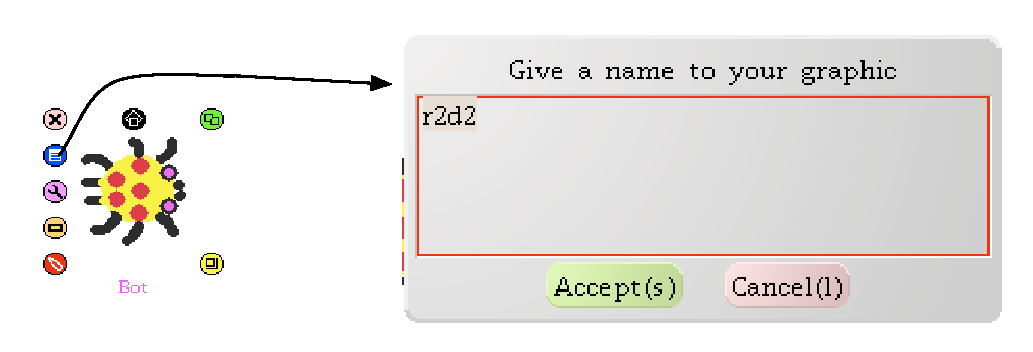
\includegraphics{nameOfSaveAnnotated}
\end{center}
\caption{Clicking on the blue handle and getting prompted for a name. \label{fig:prompt}}
\end{figure}

Doing a similar operation, you can load a graphic, by clicking on the pink halo with a tool of a robot. I used the color pink with the idea that the color pink would mean  bringing back to life your robot. When you click on the pink halo the system asks you for the name of the graphic you want to load. When the operation succeeds your robot will look like the graphic you just loaded. 

\paragraph{Involving the Class.} Now even if you drew a wonderful insect, when you will ask the class to create a new robot, you will get the default graphic. But what you can do is to tell your robot to pass its graphic to the class using the message \ct{passImageToClass}. Now if you create a new robot and ask it to look as the image, it will look as the graphic you just draw. 

Note that if you send the message \ct{lookLikeImage} or any of the lookLike message to the \emph{class} itself, the class will be configured so that the new robots will look following
the class configuration.  For example, if you send the message \ct{lookLikeCircle} to the \emph{class} \ct{Bot}, all the new robots like look like a circle. Therefore if you want to have a class creating spiders, you have to (1) get a robot, (2) draw the spider, (3) pass the spider image to the class. Then all the new robots will look like  a spider as shown by Figure~\ref{fig:allGraphics}.


\begin{figure}[h]
\begin{center}
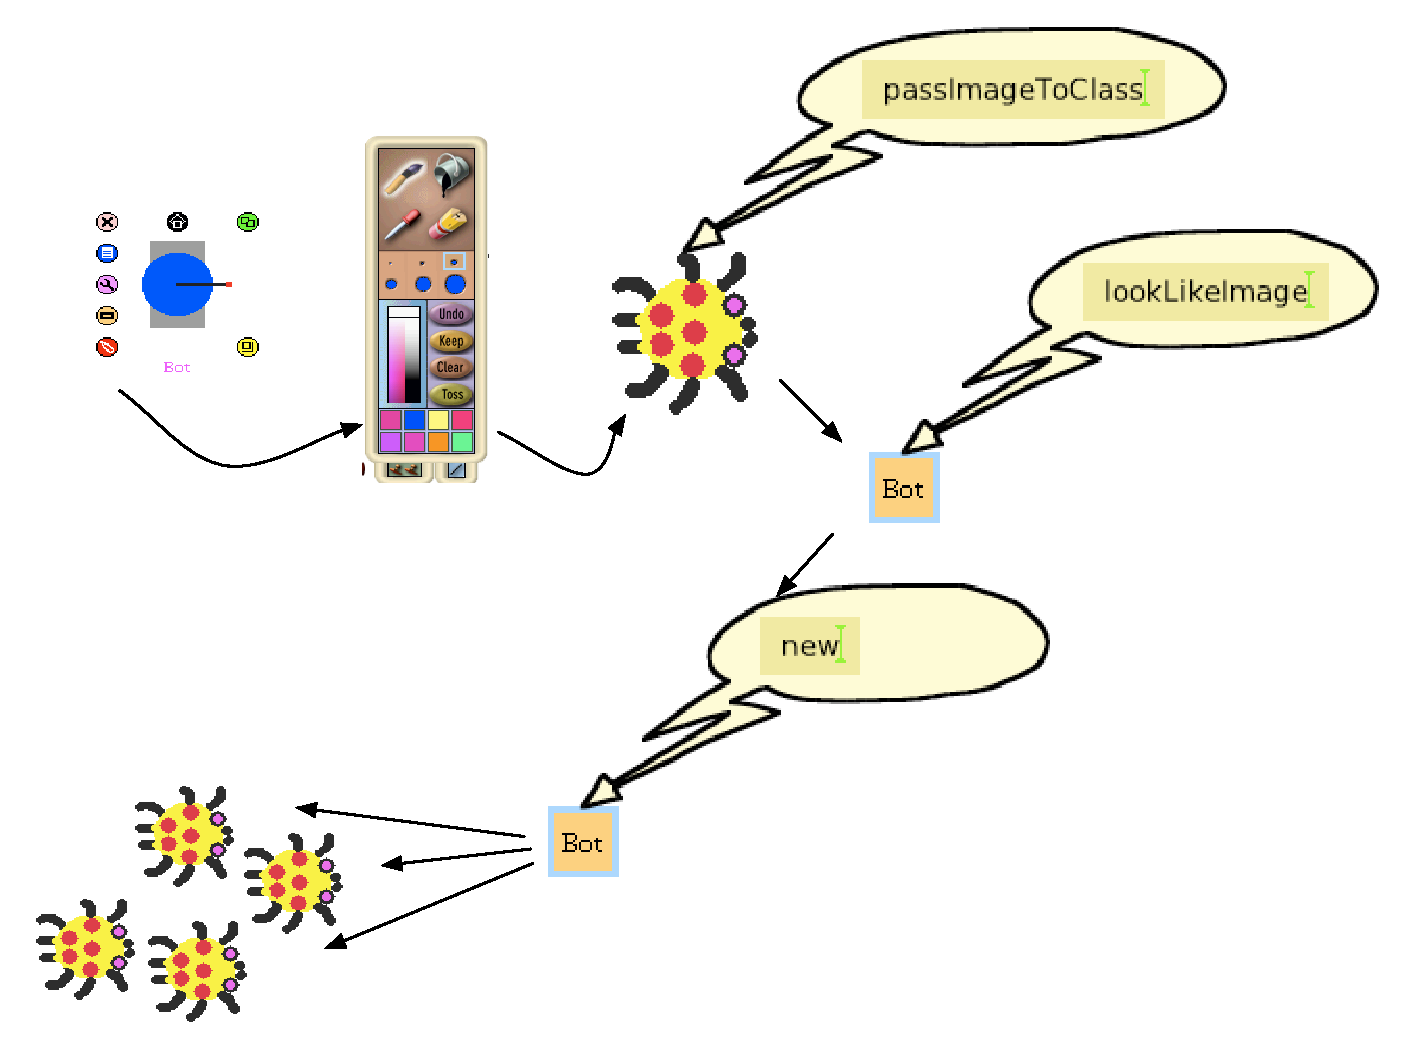
\includegraphics[width=16cm]{allGraphics2}
\end{center}
\caption{The steps to associate a new graphic to all the robots that will be created afterwards. \label{fig:allGraphics}}
\end{figure}




\subsection{Using Scripts}
You can also write scripts to load and save graphics, associating them to a single robot or to a class itself. 

Script \ref{scr:loadingGraphics} creates a robot and load a new graphic. Note that you can also use the message \ct{loadImage:} specifying the name of the file to load a specific graphic as shown by the last message which loads the graphic named \ct{spider}. Note that when you use the message \ct{loadImage: asString} you have to specify the name of the graphic with a string that is the name surrounded by single quotes. You can save the image using the methods \ct{save} or \ct{saveImage: aString} as shown in Script~\ref{scr:loadingGraphics}.


\begin{scriptwithtitle}{Loading and saving a graphic to a single robot}\label{scr:loadingGraphics}
| pica |
pica := Bot new. 
pica loadImage.
"the method loadImage prompts the user for the name of the image to load"

pica loadImage: 'spider'
"the method loadImage: requires as parameter the name of the graphic

pica saveImage: 'spider2'
"you can save the image using the methods save or saveImage:"
\end{scriptwithtitle}


Once you passed the graphics to the class, \scrref{scr:savingGraphics} shows how to use the method \index{saveImage:}\ct{saveImage: aString} to save a graphic into a file named \ct{aString}. This script creates a file named \ct{'spider.frm'} at the same location that your \sq image. You can also use the method \ct{saveImage} that will prompt you for a name. 

\begin{scriptwithtitle}{Saving the graphic associated with the class}\label{scr:savingGraphics}
Bot saveImage: 'spider2'
\end{scriptwithtitle}


The following scripts (\ref{scr:Single}, and \ref{scr:classGraphics}) have the assumption that you have saved three images named \ct{luth}, \ct{spider}, and \ct{airplane}. These files are included in the distribution of the environment used in this book. The expression \ct{Bot clearImage} clears the previously defined graphic that could be associated with the class \ct{Bot} so that you can reproduce exactly the same scenarios. Using this expression reset your environment as if you would just started it for the first time. 

\begin{scriptwithtitle}{Changing the image of one single robot}\label{scr:Single}
| pica daly |
Bot clearImage. 

pica := Bot new.
pica lookLikeImage.
"No image loaded or created so nothing changes"

pica loadImage: 'luth'.
pica lookLikeImage
"load an image and ask to look like it"

pica loadImage: 'spider'.
"load another image and as it automatically looks like 
the image the new image is shown"

daly := Bot new.
"look like a robot"
daly lookLikeImage.
"No image loaded in the class so nothing changes"
\end{scriptwithtitle}

In \scrref{scr:Single}, first there is no graphic imported so asking the robot \ct{pica} to look like an image does not produce any change. Once you load an graphic to \ct{pica} sending the message \index{loadImage:}\ct{loadImage: 'luth'} where \ct{'luth'} represents the name of the graphic file, asking \ct{pica} to look like an image produces the excepted effect. Now you control a robot that looks like a luth turtle. Note that if you read another image such as shown in the last line of the script, this image gets automatically used. 
When you create a new robot, \ct{daly}, the class does not have any graphic loaded so \ct{daly} looks like a robot and if you ask it to look like an image, nothing changes since it does not have an image.

%\scrref{scr:SingleAware} shows that up until now only one single robot got a new graphics. If you create a new robot and ask it to use a new graphics using the method \ct{lookLikeImage} nothing would happen because the class itself it not aware that there is a new graphics for the turtle. 

%
%\begin{scriptwithtitle}{Only a single robot was displaying a different graphics}\label{scr:SingleAware}
%| airplane |
%airplane := Bot new.
%airplane lookLikeImage.
%"it does not change because the class is not aware that all its 
%newly created robot should have a different graphics."
%\end{scriptwithtitle}


\scrref{scr:classGraphics} shows how to notify the class that all newly created robots can have a new graphic. Note that contrary to the situation described in \scrref{scr:Single} the message \ct{loadImage: aString} is sent to the class \ct{Bot} itself and not to a particular robot. The same message \ct{loadImage:} has different behavior depending whether it is received by different objects here a class and an instance. On a class it loads and associates the graphic so that newly created instances can use the new graphics, on a robot only the robot receiving the message can use this graphic. 


\begin{scriptwithtitle}{Associating a graphic to  the class}\label{scr:classGraphics}
| bot1 bot2 bot3 |
Bot loadImage: 'spider'.
bot1 := Bot new.
bot1 lookLikeImage
"bot1 looks now like a spider"

bot2 := Bot new.
bot2 lookLikeImage.
"bot2 looks also now like a spider"

bot3 := Bot new.
bot3 loadImage: 'luth'.
bot3 lookLikeImage.
"But a specific robot can still change its own graphics"

"To get the image of the class back"
bot3 getImageFromClass.

Bot loadImage: 'luth'.
Bot lookLikeImage.
luth := Bot new.
"Now the class will create looking like luth turtles"
\end{scriptwithtitle}

Script~\ref{scr:classGraphics} starts by loading a new graphic from a file and associates it with the class itself. Then it creates a new robot \ct{bot1} and asks it to use the new graphic. Creating another robot \ct{bot2} and performing the same procedure creates another robot with the newly imported graphic. 

All the robots created will be able to look like a spider. However a particular robot, such as the robot \ct{bot3}  in the script which look like a luth, can still have its own graphic by loading one. The method \index{getImageFromClass} \ct{getImageFromClass} allows one to restore the graphic associated with the class. The last sequence of messages shows that we can associate a new graphic to a class. Sending the message \ct{loadImage:} to the class \ct{Bot} itself associates the graphic to the class, then sending the message \ct{lookLIkeImage} makes sure that the newly created robots will look like the graphic of the class per default. Hence the robot \ct{luth} looks like the turtle. 





\summa
\begin{table}[h]
\centering
\begin{tabular}{||p{4cm}|p{7cm}|p{5cm}||} \hline
% after \\ : \hline or \cline{col1-col2} \cline{col3-col4} ...
Method&Description&Example\\[1ex] \hline
\ct{lookLikeCircle}&Change the shape of the receiver to  a circle& \ct{\Turtle new lookLikeCircle}\\ \hline
\ct{lookLikeBot}&Change the shape of the receiver to  a robot& \ct{\Turtle new lookLikeBot}\\ \hline
\ct{lookLikeTriangle}&Change the shape of the receiver to  a triangle&\ct{\Turtle new lookLikeTriangle}\\ \hline
\ct{lookLikeImage}&Change the appearance of the receiver to the graphic you painted& \ct{\Turtle new lookLikeImage} \\ \hline

\ct{lookLikeCircle}&Send to the class makes sure that the created robots will have a circle as shape& \ct{\Turtle lookLikeCircle}\\ \hline
\ct{lookLikeBot}&Send to the class makes sure that the created robots will have a robot as shape& \ct{\Turtle lookLikeBot}\\ \hline
\ct{lookLikeTriangle}&Send to the class makes sure that the created robots will have a triangle as shape&\ct{\Turtle lookLikeTriangle}\\ \hline
\ct{lookLikeImage}&Send to the class makes sure that the created robots will have a the graphic you painted or loaded as shape& \ct{\Turtle lookLikeImage} \\ \hline
\ct{loadImage: aString}&Load the image named aString in the class or the robot&\ct{\Turtle loadImage: 'spider'} or \ct{aBot loadImage: 'spider'}\\ \hline
\ct{loadImage}&Load the image named aString in the class or the robot&\ct{\Turtle loadImage} or \ct{aBot loadImage}\\ \hline
\ct{saveImage: aString}&Save the image of the class or the robot in the file named aString& \ct{\Turtle saveImage: 'spider'}  or \ct{aBot saveImage: 'spider'}\\ \hline
\ct{saveImage}&Save the image of the class or the robot by prompting the user for a name& \ct{\Turtle saveImage} or \ct{aBot saveImage} \\ \hline

\ct{penColor: aColor}&Change the color of the pen& \ct{\Turtle new penColor: Color blue}\\ \hline
\ct{penSize: aNumber}&Change the size of the pen. The default size is 1.&\ct{\Turtle new penSize: 3}\\ \hline

\ct{color: aColor}&Change the color of the receiver to the specified color& \ct{\Turtle new color: Color yellow}\\ \hline
\ct{extent: aPoint}&Change the size of the receiver. aPoint (w@h) specifies the new size of the receiver as the size of the rectangle. The first number is the width and the second the height. &\ct{\Turtle new extent: 80@100}\\ \hline

\ct{passImageToClass}&Pass the graphic of the receiver to the class. After this message, the robots created by the class will have as graphic the graphic that the current robot has.&\ct{aBot passImageToClass}\\ \hline

\ct{getImageFromClass}&Get the graphic of the class. After this message, the receiver will look like the robots that would be created by the class.&\ct{aBot getImageFromClass}\\ \hline


\end{tabular}
\end{table}

\ifx\wholebook\relax\else\end{document}\fi